\chapter{\texorpdfstring{\acrlong*{acc:ea}}{}}

Optimization. What better word would describe the ultimate goal of all the people, our civilization, and maybe even the Universe. With a bit of exaggeration, optimization is the cause of all the ramifications we can see around. Because what else are Physic laws than minimization processes, our pursuit of knowledge and self improvement than maximization of self-worth, industrial revolutions than minimization of human labour, maximization of goods production and standard of living at the same time. In my opinion, optimization is the reason what drives us forward, makes us better, and guides our decisions.

One of the most extraordinary optimization processes is, without a doubt, evolution. Evolution is nothing less than Nature way of improvement species to better adapt to their environment. The father of evolution is undoubtedly Charles, who the first come up with an idea of evolution in his work \enquote{On the origin of species: A facsimile of the first edition} \citep{darwin1964origin}. According the him, the individuals that better adapted to the environment have higher potential to reproduce and pass their genetic material --- including the predisposition to survive in the environment --- to their offsprings. Sometimes referred as \enquote{Survival of the fittest}.

This exact ideas inspired scientists and formed the field of \acrfull{acc:ea}\index{evolutionary algorithm}\footnote{I will refer to all the population-based algorithms in this work as \acrlong*{acc:ea}. These includes, among others, \acrlong*{acc:ga}, \acrlong*{acc:ea}, and \acrlong*{acc:pso}.}.
\acrshort{acc:ea} are stochastic, population-based optimization algorithms inspired by biological evolution. In general, a set of individuals called population compete with each other for a place in the next generation. Each individual represent one possible solution of the problem in hand. Quality of the individual is proportional to the quality of solution it represents. This quality is usually expressed using fitness (or sometimes called objective) function. As with natural evolution, the probability of survival is proportional the solution quality -- the better the solution is, the higher the probability of survival \citep{IntroductionToEA}. In the \acrshort{acc:ea}, the process of producing new generation is usually called selection.

Evolution is not only about survival, but also about reproduction. \acrlong*{acc:ea} took inspiration here as well and uses specials operators for each generation -- usually called evolution operators or variation operators\index{variation operator}. As the name suggests, these operators make sure the population explores new solutions. The two most common operators are crossover and mutation. During crossover\index{crossover}, individuals from the current population (usually called parents) produces new individuals (usually called offsprings) by combining their genetic information. In some way, crossover mimic reproduction in Nature, during which the \acrshort{acc:dna} of offspring is by majority determined by its parents \acrshort{acc:dna}. Mutation\index{mutation}, on the other hand, causes random small alteration of the individual genetic material and is able to introduce novel patterns that did not previously occur in the population \citep{HowToSolveItModernHeuristics}.

In general, \acrshort{acc:ea} repeat steps above until sufficiently good solution is found, or until maximum number of generations is reached. The general pseudocode of the \acrshort{acc:ea} algorithm is in Algorithm \ref{alg:SEA}. I will present more accurate implementations of various algorithms thorough this chapter.

\begin{algorithm}
    \SetAlgoLined
    \KwResult{evolved population}
    initialize population\;
    \Repeat{termination criteria met}{
        reproduction\;
        mutation\;
        evaluate population\;
        selection\;
    }
    \caption{General Evolution Algorithm}
    \label{alg:SEA}
\end{algorithm}


%%%%%%%%%%%%%%%%%%%
%%               %%
%%  TERMINOLOGY  %%
%%               %%
%%%%%%%%%%%%%%%%%%%
\section{Terminology}

In this section, I will introduce necessary terminology that I am going to use thorough this work. I took most of the terminology from \citet{IntroductionToEA}.

\defterm{Problem} is the function we want to solve. It can be both satisfactory as well optimization problem.

\defterm{Genotype}\index{genotype} is encoding of the solution. It is equivalent of the \acrshort{acc:dna} -- it compress all the data needed to produce solution.

\defterm{Gene} is one part of the genotype. It may be one bit if the genotype is encoded as binary string or scalar, if the genotype is vector. 

\defterm{Representation or genotype space} is the space of genotype.

\defterm{Phenotype}\index{phenotype} is the solution built from genotype. Genotype and phenotype can be equivalent -- for example real function optimization problem may have as a genotype vector of real numbers, that represent one of the solution. Generally, however, genotype and phenotype can be different.

\defterm{Search space} is the space of phenotype.

\defterm{Objective function} is the function the algorithm optimize. For previous example of real function optimization, the function itself can be the objective function. I will denote objective function $\objectivefn$.

\defterm{Fitness function}\index{fitness function} is the measure of quality of the solution. Note that the domain of the function is the search space. Unlike the objective function, the fitness function should guide the algorithm during the optimization. It can use the objective function directly, but other options are possible as well. For example, if the goal is to maximize objective function $\objectivefn(x)$, but the algorithm is written such that it minimize the fitness function, one may specify the fitness function as $\fitnessfn(x)=\frac{1}{\objectivefn(x)}$. I will denote fitness function $\fitnessfn$.

\defterm{Evaluation} is the process of obtaining fitness value for the genotype.

\defterm{Individual} is genotype with it's fitness value. I will denote individual by $\individual$.

\defterm{Fitness value} of individual is it's evaluation. 

\defterm{Population} is multiset of individuals -- it is possible to have same genotype in the population multiple time. However, I will still distinguish different individuals with the same genotype. I will denote the whole population as $\population$.

\defterm{Initialization} is the process of creating the first population.

\defterm{Exploitation} is the effort to use knowledge from the history in order to maximize the expected outcome \citep{SelfAdaptiveFeaturesInRealParameterEvolutionaryAlgorithms}.

\defterm{Exploration} is the effort to discover new rules about the problem in hand, although the expected outcome does not need to be the best possible. In general, the biggest problem in \acrshort{acc:ea} is the right balance between exploitation and exploration. Putting too much emphasis may cause to get stuck in the local minima, whereas putting too much focus on the exploration may cause, that the algorithm never converge. Note that \acrshort{acc:ea} is not the only field suffering from this, but for example Reinforcement Learning deals with the same problems \citep{ExplorationExploitationDilemaRL}. 

\defterm{Evolution operators} are individual steps performed each iteration.

\defterm{Selection}\index{selection} is evolution operator that picks up individuals from the current population to the next one. The selection should take into account fitness of each individual in the population and pick them proportionally. Selection therefore implements the \enquote{Survival of the fittest} law. From the mathematical point of view, selection task is to move the population into more promising area of the search space and possibly to reduce variance of the population \citep{SelfAdaptiveFeaturesInRealParameterEvolutionaryAlgorithms}. In other word, selection is exploitation step in the algorithm.

\defterm{Crossover}\index{crossover} is evolution operator, that combines some individuals (usually called \textbf{parents}) in order to create one or more new individuals (usually called \textbf{offsprings}). Offsprings are usually combination of their parents, similarly to how \acrshort{acc:dna} of the child is combination of \acrshort{acc:dna} of her parents.

\defterm{Mutation}\index{mutation} is evolution operator, that modify one individual. Mutation can be based on randomness (for example replacement of value in genotype by different value) or specialized for the problem in hand. This time the example can be \acrlong{acc:tsp}, where one possible mutation operator can \enquote{untwist} ways that cross each other. This mutation is in fact local optimization technique, as the  mutated way is shorter than the previous one \citep{TSPArticle}.

\defterm{Variation operators}\index{variation operator} are operators, that change the variation of the population, but not the mean. Variation operators are the exploration steps in the algorithm and should balance the exploitation strength of the selection. Both crossover and mutation are variation operators \citep{SelfAdaptiveFeaturesInRealParameterEvolutionaryAlgorithms}.

\defterm{Memetic operator} is operator, that uses local optimization in every iteration. Alternatively, \enquote{memetic algorithms uses local optimizer to every solution before evaluation}\citep{HowToSolveItModernHeuristics}. One of such example is the \acrlong{acc:tsp} problem mentioned earlier. Another example is the problem of searching for weights in \acrshort{acc:ann}, where one step of backpropagation algorithm is performed as part of the mutation.




%%%%%%%%%%%%%%%%%%%%%%%%%%
%%                      %%
%%  GENETIC ALGORITHMS  %%
%%                      %%
%%%%%%%%%%%%%%%%%%%%%%%%%%
\section{\texorpdfstring{\acrlong*{acc:ga}}{}}

\acrfull{acc:ga} are probably the simplest \acrfull{acc:ea} out there and as their father is usually considered \citefullauthor{HollandGA}. In the \acrshort{acc:ga}, individual are binary string of length $n$, formally
$$ \individual \in \left\{0,1\right\}^{n} $$

Fitness function maps genotype into real values
$$ \fitnessfn:\left\{0,1\right\}^{n}\rightarrow\mathbb{R} $$

The typical crossover operator is one point crossover\index{crossover!one--point}. This type of crossover require two parents and produces two offsprings. As the first step, the algorithm uniformly sample random integer $s$ in the range $\left[ 1, n-1 \right]$. The first offspring will receive genetic material up to index $s$ from the first parent, and the rest from the second one. The second offspring is created the same way, except the position of parents is exchanged. Example for $n=10$ is in figure \ref{fig:gaonepointcrossover}. In order not to modify all the individuals in the population, only $p_c\in\left[0,1\right]$ percent of individuals undergo the crossover and the children replace their parents\citep{IntroductionToEA}.

\begin{figure}
    \begin{subfigure}[b]{0.4\textwidth}
        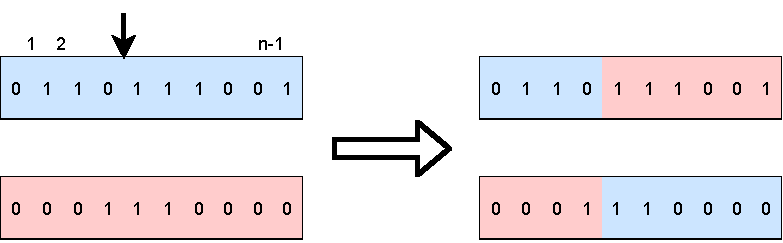
\includegraphics[width=\textwidth]{img/master_onepointcrossover.pdf}
        \caption{One point crossover}
        \label{fig:gaonepointcrossover}
    \end{subfigure}
    \hfill
    \begin{subfigure}[b]{0.4\textwidth}
        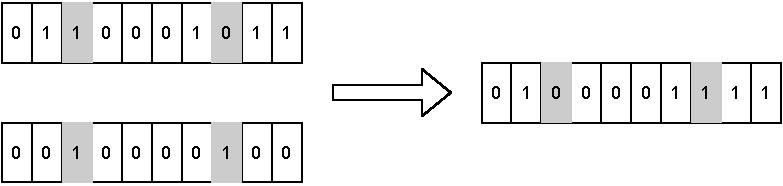
\includegraphics[width=\textwidth]{img/master_bitflipmutation.pdf}
        \caption{Bit-flip mutation}
        \label{fig:bitflipmutation}
    \end{subfigure}
    \caption{Genetic algorithm operators}
\end{figure}

The mutation\index{mutation} operator for \acrshort{acc:ga} is in most cases bit-flip mutation\index{mutation!bit-flip}. During this mutation, each gene in the genotype is mutated with probability $p_m$. One example of mutation is in figure \ref{fig:bitflipmutation}. Mutation has two objectives -- it makes sure the algorithm is not trapped in local optima, and it sustains genetic disparity in the population. As a side effect, mutation serves as minor search operator\citep{IntroToGA}.

The difference between crossover and mutation is such that crossover is rather \enquote{search} exploitation technique. It combines individuals from current population and exploit them to find possibly better individuals. Mutation, on the other hand, is more local search technique and based on the probability $p_b$ it search over the whole representation space.

Finally, the selection stage takes place. There are various selection techniques and in this particular case, I will use tournament selection\index{selection!tournament}. During tournament selection, fitness values of two random individuals are compared and the better individual is copied into the new population. This repeats as many times, as specified number of individuals form a new population.

For cases where the size of the new population equals to the size of the old one, there is high probability that the same individual will be in the following population multiple times. Nevertheless, because of crossover and mutation operators that doesn't matter, because they keep divergence in the population.

The pseudocode of simple genetic algorithm described above is depict in algorithm \ref{alg:SGA}. The population if firstly randomly initialized and then undergo crossover, mutation, evaluation, and selection operators in the loop. Finally, evolved population is returned from the algorithm.

\begin{algorithm}
    \KwIn{$d$ problem dimension, $l$ population size, $g$ generations, $\fitnessfn$, $p_c$, $p_m$}
    \KwResult{evolved population}
    population $\leftarrow$ randomnly inicialized\;
    \ForEach{$gen$ in $0$..$g$}{
        \ForEach{individual in $0$..$l$}{
            \If(){$rand()<p_c$}{One point crossover with random individual}
            \If(){$rand()<p_m$}{Bit-flip mutation}
        }
        Evaluate population using $\fitnessfn$\;
        population $\leftarrow$ pick up $l$ individuals using tournament\;
    }
    \Return{population}
    \caption{Simple genetic algorithm}
    \label{alg:SGA}
\end{algorithm}

I will refer to algorithm described above as \enquote{Simple Genetic Algorithm}. In reality, scientists come up with various operators, that can improve convergence or can help in specific types of problems. Thorough following paragraphs, I will focus on these techniques, inspired mainly by the book of authors \citet*{IntroToGA}.

\subsection{Advanced crossover operators}

Simple genetic algorithm used one point crossover. It is straightforward to extend it into two point crossover\index{crossover!two point} where each genome is split into three parts. Each offspring then receives first and third part of the genome from one parent, and the middle one from the second one. Example of two point crossover is in the picture \ref{fig:gatwopointcrossover}.

\begin{figure}
    \begin{subfigure}[b]{0.4\textwidth}
        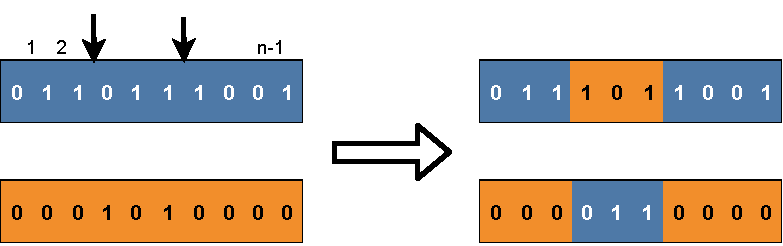
\includegraphics[width=\textwidth]{img/master_twopointcrossover.pdf}
        \caption{Two point crossover}
        \label{fig:gatwopointcrossover}
    \end{subfigure}
    \hfill
    \begin{subfigure}[b]{0.4\textwidth}
        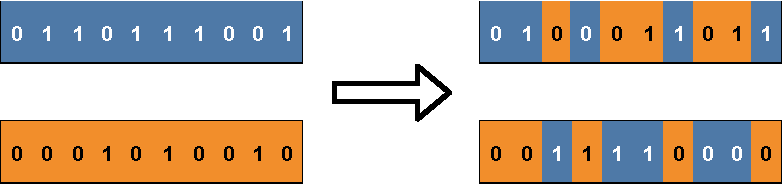
\includegraphics[width=\textwidth]{img/master_uniformcrossover.pdf}
        \caption{Uniform crossover}
        \label{fig:uniformcrossover}
    \end{subfigure}
    \caption{Advanced crossover operators}
\end{figure}

Sometimes, the crossover operator is generalized even more and forms $k$--point crossover. The genotype partitions into $k$ parts and these parts are interleaved in the offsprings. Special case is uniform crossover\index{crossover!uniform} -- the offsprings are constructed in such a way that they are uniform combination if their parents. Each gene in the offspring have equal probability whether it will be received from the first, or second parent. Second offspring will follow the same pattern, except with parents exchanged. Example of uniform crossover is in figure \ref{fig:uniformcrossover}.
% TODO Introduction into GA presents few more types - three parents crossover, crossover with reduced surrogate, and shuffle crossover. These are irrelevant for my implementation, but can be potentially described here.

\subsection{Selection operators}

